\documentclass{beamer}
\usetheme[faculty=econ]{fibeamer}

\usepackage[utf8]{inputenc}
\usepackage[francais]{babel}
\usepackage[T1]{fontenc}
\usepackage{xcolor}

\lstset{
  language=Java,                
  basicstyle=\scriptsize,
  escapeinside={*@}{*@},
  frame=single,
  xleftmargin=2mm,
  xrightmargin=2mm,
  keepspaces=true,
  tabsize=2
}

\newcounter{ctr1}
\title[]{\Large{Développement d'applications modulaires en Java}}
\author[C. Tibermacine]{\large{Chouki~Tibermacine}\\
\small{Chouki.Tibermacine@umontpellier.fr}}
%\institute{Polytech Montpellier}
\date{\tiny{}}

\begin{document}

\begin{frame}
\titlepage
\begin{flushright}

\includegraphics[width=3.5cm]{figs/polytech.png}
\end{flushright}
\end{frame}

\begin{frame}
	\frametitle{Plan de l'ECUE}
	\begin{enumerate}
		{\color{gray} \item (Rappels sur le) Développement d'applications Web avec Java
			\item Modulariser les applications Java avec Spring
		\item Bien structurer une application Web avec Spring MVC
		
			\item Auto-configurer une application Web avec Spring Boot}
			\item Sécuriser une application Web avec Spring Security
		{\color{gray}				
			\item Gérer des données massives avec Apache Kafka et Spring
			\item Tester une application Web Spring
			\item Écrire des applications Web (API) réactives avec Spring WebFlux}
	\end{enumerate}
\end{frame}

\AtBeginSection[]{% Print an outline at the beginning of sections
  \begin{frame}<beamer>
    \frametitle{Plan du cours}
    % \frametitle{Outline}
    \tableofcontents[currentsection]
    % \tableofcontents
  \end{frame}}

\AtBeginSubsection[]{% Print an outline at the beginning of sections
  \begin{frame}<beamer>
    \frametitle{Plan du cours}
    % \frametitle{Outline}
    \tableofcontents[currentsubsection]
    % \tableofcontents
  \end{frame}}

\section{Intro à la sécurité des app Web avec Spring}

\begin{frame}
  \frametitle{Besoins en sécurité}
	\begin{tikzpicture}[overlay,remember picture]
	\node[anchor=center,xshift=0pt,yshift=0pt]
	at (current page.center) {
		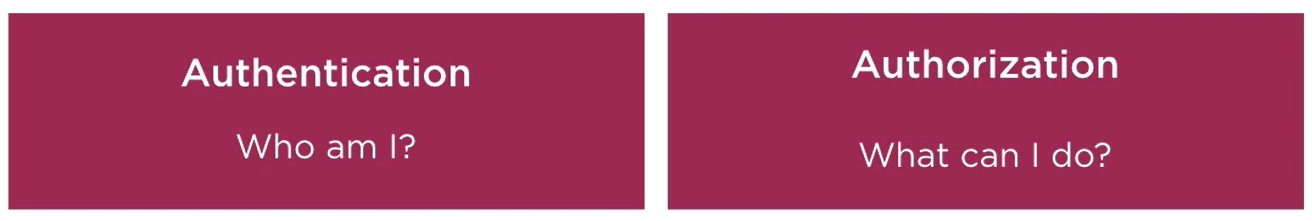
\includegraphics[width=12cm]{img/authen_author.png}
	};
\end{tikzpicture}
\end{frame}

\begin{frame}
	\frametitle{Features de \textit{Spring Security}}
	\begin{itemize}
		\item \textit{Spring Security} : framework construit au dessus de Spring
		\item Il s'intègre bien avec un CAS, des tokens OAuth, LDAP, ou des bases de données d'utilisateurs
		\item Il est basé sur la notion de Filter (sevlets) comme point d'entrée (mécanisme interne au framework)
		\item Il gère de multiples modèles d'authentification (\textit{in-memory}, \textit{database}, ...)
		\item Il encourage l'utilisation de sels (\textit{salts}) 
		\item Il fournit une liste assez importante de features pour gérer l'authentification \& l'autorisation et leur personnalisation (perte de mots de passe, par exemple), ce qui simplifie la sécurisation d'une app Web Java
	\end{itemize}
\end{frame}

\begin{frame}[fragile]
	\frametitle{Dépendances vers \textit{Spring Security}}
\begin{itemize}
	\item Déclarer l'utilisation de Spring Security dans le script de build Gradle~:
\begin{lstlisting}
implementation('org.springframework.boot:spring-boot-starter-security')
testImplementation('org.springframework.security:spring-security-test')
\end{lstlisting}
\item Pour les besoins de l'exemple ci-après, nous allons déclarer l'utilisation d'un compilateur JSP
\begin{lstlisting}
runtimeOnly('org.apache.tomcat.embed:tomcat-embed-jasper')
\end{lstlisting}
\end{itemize}
\end{frame}

\begin{frame}[fragile]
	\frametitle{Un premier exemple}
	\begin{itemize}
\item Nous allons ajouter une classe de configuration de la sécurité et l'annoter d'une certaine façon pour qu'elle soit prise en compte par le framework (la mettre dans le package racine de votre app)
\begin{lstlisting}
@Configuration
@EnableWebSecurity
public class CovidAlertSecurityConfig extends WebSecurityConfigurerAdapter {
	...
}
\end{lstlisting}
	\end{itemize}
\end{frame}

\begin{frame}[fragile]
	\frametitle{Définition de la sécurité -- \textit{Builder pattern}}
	\begin{itemize}
		\item Dans la classe précédente, on redéfinit la méthode suivante~:
	\end{itemize}		
\begin{lstlisting}
protected void configure(final HttpSecurity httpSecurity) throws  Exception {
	httpSecurity
	.authorizeRequests()
	.antMatchers("/login*").permitAll()
	.antMatchers("/static/css/**","/static/js/**",
	             "/images/**").permitAll()
	.antMatchers("/index*").permitAll()
	.anyRequest().authenticated()
	.and().formLogin().loginPage("/login")	
	.loginProcessingUrl("/doLogin")
	.failureUrl("/login?error=true").permitAll()
	.defaultSuccessUrl("/",true);
}
\end{lstlisting}
Lire chaque ligne et se documenter sur son rôle\\
Pas besoin de définir la vue \texttt{doLogin}. Les requêtes qui visent cette vue sont traitées par les filtres Spring Security
\end{frame}

\begin{frame}[fragile]
	\frametitle{Un premier exemple -suite-}
	\begin{itemize}
		\item Toujours dans la classe précédente, on ajoute les méthodes suivantes~:
\begin{lstlisting}
protected void configure(final 
  AuthenticationManagerBuilder auth) throws Exception {
	auth.inMemoryAuthentication()
	.withUser("bob").password(passwordEncoder()
	.encode("password_de_bob")).roles("USER");
}

@Bean
public PasswordEncoder passwordEncoder() {
	return new BCryptPasswordEncoder();
}
\end{lstlisting}
Cela permet de déclarer un premier utilisateur (\textit{bob}) dans l'application, avec un mot de passe encodé avec la fonction de hachage \texttt{BCrypt}, et lui donner le rôle de \texttt{USER}
	\end{itemize}
\end{frame}

\begin{frame}[fragile]
	\frametitle{Côté contrôleur}
	Une classe Contrôleur comme solveur des vues
\begin{lstlisting}
@Controller
public class ViewController {
	@GetMapping({"/", "/index"})
	public String home() { return "index"; }
	
	@GetMapping({"/login"})
	public String login() {	return "login"; }

	@GetMapping({"/changeUser"})
	public String changeUser() { return "changeUser"; }

	@GetMapping({"/listUsers"})
	public String listUsers() { return "listUsers"; }
}
\end{lstlisting}
Dans \texttt{application.properties}, ajouter~:\\
\footnotesize
\texttt{spring.mvc.view.prefix=/WEB-INF/jsp/\\
	spring.mvc.view.suffix=.jsp}
\normalsize
\end{frame}

\begin{frame}[fragile]
	\frametitle{Côté Front-end}
Dans une page JSP (login.jsp)~: (fournie dans le dépôt Git)
\begin{lstlisting}
<div class="container">
 <h1>Login</h1>
 <% if(request.getParameter("error") != null) { %>
  <div class="errblock">Invalid Username and Password</div>
 <% } %>
 <form:form action="/doLogin" method="POST">
  <label for="username">User name: </label>
  <input type="text" id="username" name="username"/>
  <br/>
  <label for="password">Mot de passe</label>
  <input type="password" id="password" name="password"/>
  <br/>
  <input type="submit" value="Login" role="button" class="btn btn-lg btn-primary" />
 </form:form>
</div>
\end{lstlisting}
La placer dans le dossier src/main/webapp/WEB-INF/jsp/
\end{frame}

\section{Sécuriser en utilisant différentes sources de données}

\begin{frame}[fragile]
	\frametitle{Une source de données \textit{in-memory}, LDAP, ...}
	\begin{itemize}
		\item \textit{In-memory}, utilisé dans l'exemple précédent~:
\begin{lstlisting}
auth.inMemoryAuthentication()
    .withUser("bob").password(passwordEncoder()
    .encode("password_de_bob")).roles("USER");
\end{lstlisting}
\item Il est possible également d'utiliser LDAP. Pour cela, il faudra~:

\begin{itemize} 
\item ajouter de nouvelles dépendances Spring Security LDAP
\item configurer les paramètres de connexion au service LDAP (dans \textit{application.properties})
\end{itemize}
\end{itemize}

\end{frame}

\begin{frame}[fragile]
	\frametitle{Une source de données \textit{in-memory}, LDAP, ...}
	\begin{itemize}
		\item Utiliser LDAP~: -suite-
		\begin{itemize}		
			\item personnaliser la configuration en indiquant~:
\begin{lstlisting}
auth.ldapAuthentication()
	.userDnPatterns("uid={0},ou=people")
	.groupSearchBase("ou=groups")
	.contextSource()
	.url("ldap://...:8389/dc=iwa,dc=fr")
	.and()
	.passwordCompare()
	.passwordEncoder(passwordEncoder())
	.passwordAttribute("userPassword")
\end{lstlisting}
\end{itemize}
	\end{itemize}
\end{frame}

\begin{frame}[fragile]
	\frametitle{Une source de données externe}
	\begin{itemize}
		\item Une base de données qui contient  la table des utilisateurs
		\item Dans la classe de configuration de la sécurité~:		
	\end{itemize}
\begin{lstlisting}
@Configuration
@EnableWebSecurity
public class CovidAlertSecurityConfig extends WebSecurityConfigurerAdapter {
 @Autowired
 DataSource dataSource;
 // ... configure() method with security definition
 @Override
 protected void configure(final 
  AuthenticationManagerBuilder auth) throws Exception {
  auth.jdbcAuthentication().passwordEncoder(passwordEncoder()).dataSource(dataSource)
  .withUser("admin").password(passwordEncoder().encode("adminadmin")).disabled(false).roles("USER","ADMIN");
 } }
\end{lstlisting}
Config de Postgres identique au cours précédent
	
\end{frame}

\begin{frame}[fragile]
	\frametitle{Côté Postgres}
	\begin{itemize}
		\item Mettre à jour la table users (la table doit s'appeler ainsi) en ajoutant~:
\begin{lstlisting}[language=Sql]
username varchar(50) NOT NULL PRIMARY KEY,
password varchar(100) NOT NULL,
enabled boolean NOT NULL DEFAULT false
\end{lstlisting}	
et en supprimant les contraintes NOT NULL pour les autres champs. Par exemple, dans le Shell \texttt{psql}~:\\
\footnotesize
\texttt{alter table users alter column email drop not null;}	
\normalsize
\item Ajouter la table suivante~:
\begin{lstlisting}[language=Sql]
CREATE TABLE authorities(
  authority_id serial primary key,
  username varchar(50) NOT NULL 
           REFERENCES users (username),
  authority varchar(50) NOT NULL DEFAULT 'ROLE_USER'
);
\end{lstlisting}		
	\end{itemize}
\end{frame}

\begin{frame}[fragile]
	\frametitle{Tester cela}
	\begin{itemize}
		\item Modifier la base de données Postgres comme expliqué ci-haut
		\item Insérer quelques utilisateurs dans les deux tables~:
		\begin{itemize}
			\item Pour obtenir l'encodage en \texttt{BCrypt} d'un mot de passe, utiliser la classe de test de votre projet Gradle~: déclarer dans cette classe un attribut auto-injecté (\texttt{@Autowired}) de type \texttt{PasswordEncoder} et, dans la méthode de test (\texttt{contextLoads()}), faire un \texttt{print} du résultat retourné par la méthode encode invoquée sur ce bean (auto-injecté)
			\item Faire un \textit{Run} de cette classe (clique bouton droit, puis Run)
			\item Autre option : outils en ligne, comme \url{https://bcrypt-generator.com/}
		\end{itemize}
		\item Changer la configuration \texttt{in-memory} par une config. JDBC
	\end{itemize}
\end{frame}

\begin{frame}[fragile]
\frametitle{Tester cela -suite}
\begin{itemize}		
		\item Modifier la classe Entity \texttt{User} pour refléter les changements faits dans la base de données (champs username, password et enabled)
		\item Ajouter une nouvelle classe Entity Authority qui correspond à la table \texttt{authorities}
		\item Démarrer Postgres si ce n'est pas déjà fait, puis démarrer l'app
		\item Pour suivre l'évolution du système d'authentification, avec ses différents filtres mis en place, les exceptions qui sont levés et capturés pour déclencher l'authentification, ajouter la ligne suivante dans \texttt{application.properties}~:\\
\begin{lstlisting}
logging.level.org.springframework.security=DEBUG
\end{lstlisting}
Les logs sont visibles dans la console du serveur (sur votre IDE)
	\end{itemize}
\end{frame}

\section{Personnaliser le processus d'authentification}

\begin{frame}[fragile]
	\frametitle{Remember Me}
	\begin{itemize}
		\item On aimerait que l'application se rappelle d'un utilisateur déjà authentifié
		\item Nous allons d'abord ajouter une case à cocher dans le formulaire d'authentification que l'utilisateur peut cocher~:
\begin{lstlisting}[language=Html]
<label>Remember me: 
  <input type="checkbox" name="remember-me">
</label>
\end{lstlisting}
\item Ensuite, nous personnalisons la méthode \\
\footnotesize\texttt{configure(final HttpSecurity httpSecurity)}~:\normalsize
\begin{lstlisting}
...
.defaultSuccessUrl("/",true)
.and()
.rememberMe()
.key("cleSuperSecrete")
.tokenRepository(tokenRepository())
\end{lstlisting}
	\end{itemize}
\end{frame}

\begin{frame}[fragile]
	\frametitle{Remember Me -suite-}
	\begin{itemize}
		\item Nous allons ajouter la méthode \texttt{tokenRepository()} invoquée avant :
\begin{lstlisting}
@Bean
public PersistentTokenRepository tokenRepository() {
	JdbcTokenRepositoryImpl token = new JdbcTokenRepositoryImpl();
	token.setDataSource(dataSource);
	return token;
}
\end{lstlisting}
	\end{itemize}
\end{frame}

\begin{frame}[fragile]
	\frametitle{Remember Me - côté Postgres}
	\begin{itemize}
		\item Ajouter la table suivante dans laquelle les tokens sont générés~:
\begin{lstlisting}[language=Sql]
CREATE TABLE persistent_logins(
 username varchar(50) NOT NULL 
          REFERENCES users (username),
 series varchar(64) PRIMARY KEY,
 token varchar(64) NOT NULL,
 last_user timestamp NOT NULL
)
\end{lstlisting}
\item Tester cette fonctionnalité
\item Un nouvel enregistrement est ajouté dans cette table si on coche la case ``\textit{Remember Me}''
\item Même au redémarrage du serveur, l'utilisateur reste authentifié
	\end{itemize}
\end{frame}

\begin{frame}[fragile]
	\frametitle{Se déconnecter (\textit{logout})}
	\begin{itemize}
		\item Personnaliser la méthode configure, en ajoutant~:
\begin{lstlisting}
...
.and()
.logout()
.logoutSuccessUrl("/login?logout=true")
.logoutRequestMatcher(
	new AntPathRequestMatcher("/doLogout","GET")
)
.invalidateHttpSession(true)
.deleteCookies("JSESSIONID")
.permitAll();
\end{lstlisting}
\item Ici>, les requêtes vers la vue \texttt{doLogout} sont gérées par les filtres Spring Security (pas besoin donc de la définir)
	\end{itemize}
\end{frame}

\begin{frame}[fragile]
	\frametitle{Côté Front-end}
	\begin{itemize}
		\item Dans la vue de login~:
\begin{lstlisting}
<% if(request.getParameter("logout") != null) { %>
  <div class="alert alert-success" role="alert">
  	Logout was successful
  </div>
<% } %>
\end{lstlisting}
		\item N'importe où dans les vues de l'application, ajouter la possibilité de faire un \textit{logout}
\begin{lstlisting}[language=Html]
<a href="/doLogout">Logout</a>
\end{lstlisting}				
		
	\end{itemize}
\end{frame}

\section{Gérer le processus d'enregistrement d'utilisateurs}

\begin{frame}
	\frametitle{Le processus d'enregistrement}
	\begin{itemize}
		\item Le processus d'enregistrement d'un nouvel utilisateur est le suivant~:
		\begin{enumerate}
			\item L'utilisateur remplit le formulaire d'inscription et valide
			\item L'application envoie un email de confirmation, avec un lien
			\item L'utilisateur confirme la création de son compte, en cliquant sur le lien
		\end{enumerate}		
		\item Ajouter au formulaire d'enregistrement des utilisateurs de votre application, un champ de mot de passe et un deuxième champ de confirmation du mot de passe (les attributs ``\texttt{name}" des champs les plus importants pour la suite du cours doivent avoir comme valeurs~: username et password)
		\item Pour l'envoi d'emails, utiliser un compte Gmail, mais vous devez activer l'option d'utilisation de ce compte par les applications ("Less Secure Apps") dans les paramètres de config Gmail
	\end{itemize}
\end{frame}

\begin{frame}[fragile]
	\frametitle{Côté Backend}
	Prévoir les méthodes nécessaires dans le contrôleur (solveur de vues) : 
	\begin{enumerate}
		\item \texttt{register} pour l'accès à la vue qui fournit le formulaire~: \\
		Récupérer le fichier register.jsp sur le dépôt Git
		\item \texttt{doRegister} pour le traitement des données du formulaire (voir ci-après)
	\end{enumerate}		

\end{frame}

\begin{frame}[fragile]
\frametitle{Côté Backend -suite-}
\begin{itemize}	
		\item La seconde méthode du contrôleur~:
\end{itemize}		
\begin{lstlisting}
@PostMapping("doRegister")
public String register(@Valid @ModelAttribute("user")
			  User user, BindingResult result) {
 // check for errors ...
 // verify that username does not exist:
 if(userRepository.existsUserByUsername(user.getUsername())) {
  return "register.jsp?user=true";
 }
 else {	// encrypt password:
  user.setPassword(passwordEncoder.encode(user.getPassword()));
  // save user object:
  userRepository.saveAndFlush(user);
  // create/save an Authority obj ...  
  return "login";
 }
}
\end{lstlisting}		
	
\end{frame}

\begin{frame}[fragile]
	\frametitle{Côté Backend -suite-}
	\begin{itemize}
		\item Dans la méthode précédente, nous avons utilisé le bean \texttt{userRepository}. Celui-ci doit être déclaré comme attribut auto-injecté dans la classe~:
\begin{lstlisting}
@Autowired
private UserRepository userRepository;
\end{lstlisting}	
De même pour \texttt{authorityRepository} (dont la classe doit être créée en même temps que la classe \texttt{Entity Authority})
		\item Nous avons également utilisé le bean \texttt{passwordEncoder}. Celui-ci doit être déclaré de la même façon~:
\begin{lstlisting}
@Autowired
private PasswordEncoder passwordEncoder;
\end{lstlisting}		
\end{itemize}
\end{frame}

\begin{frame}[fragile]
\frametitle{Côté Backend -suite-}
\begin{itemize}
		\item Nous avons également utilisé une méthode \texttt{existsUserByUsername}, qui n'existe pas encore dans le bean \texttt{userRepository}. Il faudra l'ajouter à l'interface \texttt{UserRepository} définie dans le cours précédent (interface \textit{JPA Repository})~:
\begin{lstlisting}
boolean existsUserByUsername(String username);
\end{lstlisting}
Spring fournira l'implem de cette méthode en cherchant parmi les entities de type \texttt{User} un objet qui a le \texttt{username} passé en argument (respecter le nommage comme ci-dessus)
\item La méthode ajoutée ci-dessus complète l'interface, qui contient par défaut une méthode \texttt{existsById()} qui prend en argument un Id de type long, ce qui n'est pas approprié pour l'exemple
	\end{itemize}
\end{frame}

\begin{frame}[fragile]
	\frametitle{Côté Front-end}
	\begin{itemize}
		\item Nous allons prévoir dans la vue, qui présente la formulaire, un bloc pour l'affichage du message d'erreur si jamais un utilisateur existe avec le même nom~:
\begin{lstlisting}
<% if(request.getParameter("user") != null) { %>
<div class="errorblock">A user with the same username already exists</div>
<% } %>
\end{lstlisting}
	\end{itemize}
\end{frame}

\begin{frame}[fragile]
	\frametitle{Envoi de mail}
	\begin{itemize}
		\item L'envoi de mail doit se faire, de préférence, en mode asynchrone
		\item Nous allons voir comment le faire avec des événements
		\item D'abord ajouter la dépendance suivante~:
\begin{lstlisting}
implementation('org.springframework.boot:spring-boot-starter-mail')
\end{lstlisting}		
\item Ensuite indiquer la config du serveur mail (SMTP) dans le fichier \texttt{application.properties}
\begin{lstlisting}
spring.mail.host=smtp.gmail.com
spring.mail.port=587
spring.mail.username=<votre-username>@gmail.com
spring.mail.password=<votre-mot-de-passe>
spring.mail.properties.mail.smtp.auth=true
spring.mail.properties.mail.smtp.starttls.enable=true
\end{lstlisting}
	\end{itemize}
\end{frame}

\begin{frame}[fragile]
	\frametitle{Définition de l'événement}
	\begin{itemize}
		\item Créer une classe dans un sous-package \texttt{util}, qui s'appelle \texttt{OnCreateUserEvent}
		\item Cette classe doit étendre \texttt{org.springframework.context.ApplicationEvent}~:
	\end{itemize}
\begin{lstlisting}
public class OnCreateUserEvent extends ApplicationEvent {
 private String appUrl; private User user;
 public OnCreateUserEvent(String appUrl, User user) {
  super(user);
  this.appUrl = appUrl;
  this.user = user;
 }
 public String getAppUrl() {
  return appUrl;
 }
 public User getUser() {
  return user;
 }
}
\end{lstlisting}
\end{frame}

\begin{frame}[fragile]
	\frametitle{Mise à jour du contrôleur}
	Pour signaler l'événement, nous allons modifier le contrôleur qui gère le POST~:
	\begin{itemize}
		\item Ajouter d'abord un attribut auto-injecté~:
\begin{lstlisting}
@Autowired
private ApplicationEventPublisher eventPublisher;
\end{lstlisting}
\item Ensuite, nous allons déclencher l'événement~:
\begin{lstlisting}
@PostMapping("doRegister")
public String register(@Valid @ModelAttribute("user")
       User user, BindingResult result) {
  ...
  // Dans le else
  eventPublisher.publishEvent(new OnCreateUserEvent("/",user));
}
\end{lstlisting}
	\end{itemize}
\end{frame}

\begin{frame}[fragile]
	\frametitle{Définition de l'écouteur d'événement}
	\begin{itemize}
		\item Créer une classe dans le package \texttt{util} 
\begin{lstlisting}
@Component
public class UserListener implements ApplicationListener<OnCreateUserEvent> {
 @Override
 public void onApplicationEvent(OnCreateUserEvent event) {
 	this.confirmCreateUser(event);	
 }
}
\end{lstlisting}
	\end{itemize}
\end{frame}

\begin{frame}[fragile]
	\frametitle{Définition de l'écouteur d'événement -suite-}
	\begin{itemize}
		\item Ajouter dans la classe précédente~:
	\end{itemize}
\begin{lstlisting}
// Ceci peut etre fait dans application.properties
private String serverUrl = "http://localhost:8080";
@Autowired
private JavaMailSender mailSender;
private void confirmCreateUser(OnCreateUserEvent event) {
 // get the user
 User user = event.getUser();
 // create verification token
 String token = UUID.randomUUID().toString();
 VerificationToken verifToken = new VerificationToken();
 // VerificationToken est une classe qu'on va definir apres
 verifToken.setToken(token);
 verifToken.setUsername(user.getUsername());
 verifToken.setExpiryDate(verifToken.calculateExpiryDate(VerificationToken.EXPIRATION));
 verificationTokenRepository.saveAndFlush(verifToken);
 // ...	
}
\end{lstlisting}
	
\end{frame}

\begin{frame}[fragile]
	\frametitle{Définition de l'écouteur d'événement -suite-}
	\begin{itemize}
		\item Toujours dans la classe précédente~:
	\end{itemize}
\begin{lstlisting}
...
private void confirmCreateUser(OnCreateUserEvent event) {
 // get email properties
 String recipientAddesss = user.getEmail();
 String subject = "User Account Confirmation";
 String confirmationUrl = event.getAppUrl()+"userConfirm?token="+token;
 String message = "Please confirm:";
 // send email
 SimpleMailMessage email = new SimpleMailMessage();
 email.setTo(recipientAddesss);
 email.setSubject(subject);
 email.setText(message+"\r\n"+serverUrl+confirmationUrl);
 mailSender.send(email);
}
\end{lstlisting}

\end{frame}

\begin{frame}[fragile]
	\frametitle{Définition de l'écouteur d'événement -suite-}
	\begin{itemize}
		\item Créer une classe dans le package \texttt{models} pour gérer les tokens
	\end{itemize}
\begin{lstlisting}
@Entity(name="verif_tokens")
public class VerificationToken {
	public static final int EXPIRATION = 60 * 24; // nb min
	@Id
	private String token;
	private String username;
	private Date expiryDate;
	public Date calculateExpiryDate(int expiryTimeInMinutes) {
		Calendar cal = Calendar.getInstance();
		cal.add(Calendar.MINUTE,expiryTimeInMinutes);
		return cal.getTime();
	}
	// + getters and setters
}
\end{lstlisting}
Ajouter une table avec les 3 champs et l'interface JPA repository VerificationTokenRepository
\end{frame}

\begin{frame}[fragile]
	\frametitle{Confirmation de la création du compte utilisateur}
	\begin{itemize}
		\item Pour confirmer la création du compte utilisateur, on a besoin juste d'afficher~:
\begin{lstlisting}[language=Html]
<div class="alert alert-success" role="alert">
  Your user account has been created
</div>
\end{lstlisting} 
\item Mais il faudrait également vérifier un certain nombre de choses avant
\item D'abord, nous allons mettre à jour le contrôleur pour prendre en charge la requête correspondant à l'URL envoyé à l'utilisateur
\item Le code qui va être défini dans le contrôleur peut être déplacé dans une méthode définie dans une classe \texttt{@Service} pour que le contrôleur soit déchargé de cette ``logique métier''
	\end{itemize}
\end{frame}

\begin{frame}[fragile]
	\frametitle{Prendre en charge la requête}
	\begin{itemize}
		\item Le contrôleur de la requête~:
	\end{itemize}
\begin{lstlisting}
@GetMapping({"/userConfirm"})
public String confirmUser(@RequestParam("token") String token) {
 VerificationToken verifToken = verificationTokenRepository.getOne(token);
 if(verifToken != null) {
  Date date = Calendar.getInstance().getTime();
  if(date.before(verifToken.getExpiryDate())) {
   verificationTokenRepository.delete(verifToken);
   User user = userRepository.findByUsername(verifToken.getUsername());
   user.setEnabled(true);
   userRepository.saveAndFlush(user);
   return "login.jsp?confirm=true";
  }
\end{lstlisting}
\end{frame}

\begin{frame}[fragile]
\frametitle{Prendre en charge la requête -suite-}
\begin{itemize}
	\item Suite de la méthode du contrôleur~:

\end{itemize}	
\begin{lstlisting}
  else {
   verificationTokenRepository.delete(verifToken);
   return "register.jsp?expired=true";
  }
 }
 else { return "register.jsp?confirm=false"; }
}
\end{lstlisting}
Plus haut, nous avons utilisé une nouvelle méthode \texttt{findByUsername()}. Il faut ajouter la signature suivante à l'interface UserRepository (Spring fournit l'implem qu'il faut)~:\\
\texttt{User findByUsername(String username);}
\end{frame}

\begin{frame}[fragile]
\frametitle{Prendre en charge la requête -suite-}
\begin{itemize}
	\item Prévoir les messages d'erreur dans \texttt{register.jsp}. Exemple~:
\begin{lstlisting}
<% if(request.getParameter("expired") != null) { %>
 <div class="errorblock">The registration has expired. Please re-sign-up</div>
<% } %>
\end{lstlisting}
	\item Prévoir le message de succès dans la vue \texttt{login.jsp}~:
\begin{lstlisting}
<% if(request.getParameter("confirm") != null) { %>
 <div class="alert alert-success" role="alert">User creation is confirmed. Please log in</div>
<% } %>
\end{lstlisting}
	\item Prévoir d'ajouter la nouvelle route (\texttt{/userConfirm}) dans la méthode \texttt{configure} de définition de la sécurité pour autoriser l'accès sans authentification à cette vue~:
\begin{lstlisting}
.antMatchers("/userConfirm").permitAll()
\end{lstlisting}
	\end{itemize}
\end{frame}

\begin{frame}[fragile]
	\frametitle{Mise en place de la fonctionnalité ``Oubli du mot de passe''}
	\begin{itemize}
		\item Ajouter un lien dans la page de login~: \textit{Forgot Password}
		\item Ajouter un formulaire pour saisir le \texttt{username} et l'\texttt{email}
		\item Ajouter le contrôleur nécessaire qui permet d'envoyer un email (\textit{Reset Password}) avec un lien (incluant un token qui expire, comme précédemment) pour la mise à jour du mot de passe
		\item Mettre en place la mise à jour du mot de passe (vue + contrôleur)
	\end{itemize}
\end{frame}

\section{Sécuriser les méthodes et les éléments du Front}

\begin{frame}[fragile]
	\frametitle{Sécuriser les méthodes}
	\begin{itemize}
		\item D'abord, ajouter une annotation sur la classe de config de la sécurité~:
\begin{lstlisting}
@EnableGlobalMethodSecurity(
  prePostEnabled=true,
  securedEnabled=true,
  jsr250Enabled=true
)
\end{lstlisting}
Ceci permet d'activer les annotations prePost pour gérer plus finement l'avant et l'après exécution d'une méthode, les annotations Spring (deuxième true) et les annotations standards Java
\item Ces annotations sont désactivées, par défaut
	\end{itemize}
\end{frame}

\begin{frame}[fragile]
\frametitle{Sécuriser les méthodes -suite-}
\begin{itemize}
		\item Ensuite, on peut annoter une méthode en particulier, en indiquant le rôle de l'utilisateur qui a le droit d'exécuter la méthode (après s'être authentifié)~:
\begin{lstlisting}
@PostMapping("/listUsers")
@Secured("ROLE_ADMIN")
public String listUsers() {
	...
}
\end{lstlisting}	
\texttt{@Secured} est une annotation Spring activée par \texttt{securedEnabled}
\item Si on teste cela, lorsqu'un utilisateur, avec le rôle \texttt{USER} seulement, clique sur le lien pour lister les utilisateurs, il reçoit une réponse HTTP 403 (\textit{Forbidden})
	\end{itemize}
\end{frame}

\begin{frame}[fragile]
	\frametitle{Sécuriser les éléments du Front}
	\begin{itemize}
		\item Pour cacher par exemple le lien "List Users" à l'utilisateur s'il n'est pas ADMIN
		\item Cela se fait simplement avec des balises spéciales de Spring Security qui vont entourer les éléments du Front à sécuriser
		\item D'abord, ajouter la dépendance au script de build~:
\begin{lstlisting}
implementation('org.springframework.security:spring-security-taglibs')
\end{lstlisting}
\item Ensuite, dans une vue (\texttt{index.jsp}, par exemple) nous allons importer la taglib~:
\begin{lstlisting}
<%@ taglib prefix="sec" uri="http://www.springframework.org/security/tags" %>
\end{lstlisting}
	\end{itemize}
\end{frame}

\begin{frame}[fragile]
	\frametitle{Sécuriser les éléments du Front}
	\begin{itemize}
		\item Afficher un élément si un utilisateur est authentifié ou pas~:
\begin{lstlisting}[language=Html]
<sec:authorize access="! isAuthenticated()">
 <a href="/login">Log in</a><br/>
 <a href="/register">Create a User Account</a><br/>
</sec:authorize>
<sec:authorize access="isAuthenticated()">
 <a href="/changeUser">Change User Account</a><br/>
 <a href="/listUsers">List User Accounts</a>
</sec:authorize>
\end{lstlisting}
\item Afficher le nom de l'utilisateur authentifié~:
\begin{lstlisting}[language=Html]
<sec:authentication property="principal.username"/>
\end{lstlisting}
\item Dans les méthodes des contrôleurs, nous avons la possibilité d'ajouter un dernier paramètre de type \texttt{Authentication}. Cet objet (injecté) fournit une méthode \texttt{getPrincipal()} qui retourne un objet comportant le username, password, rôles, ...
	\end{itemize}
\end{frame}

\section{Conclusion : synthèse et ajustements supplémentaires}

\begin{frame}[fragile]
	\frametitle{\textit{Wrap-up}}
	\begin{itemize}
		\item Spring Security protège votre application des attaques classiques comme CSRF et XSS, grâce à~: i)~un HTTP Firewall, ii)~des filtres de contrôle implicites activés par défaut avant le servlet dispatcher, et ~iii)~des tokens supplémentaires
		\item En inspectant les headers des réponses HTTP de votre app~:
\begin{lstlisting}
Cache-Control: no-cache; ...
X-Content-Type-Options: nosniff
X-XSS-Protection: 1; mode=block
\end{lstlisting}
		\item Ces filtres sont désactivables dans \texttt{configure(HttpSecurity http)}~: \texttt{.headers().defaultsDisabled()} ou \texttt{.csrf().disable()}, mais ce n'est pas ce qui est recommandé
	\end{itemize}
\end{frame}


\begin{frame}[fragile]
\frametitle{\textit{Wrap-up} -suite- : derniers ajustements}
\begin{itemize}		
		\item Pour activer HTTPS dans votre app Spring Boot~: \footnotesize \url{https://www.tutorialspoint.com/spring_boot/spring_boot_enabling_https.htm}
		\normalsize
		\item Le tuto ci-dessus explique comment générer et utiliser un certificat auto-signé. Le navigateur vous demandera d'accepter l'exception de sécurité
		\item Pour générer un certificat fourni par une autorité de certification reconnue par les navigateurs, compléter votre app~:\\
		\footnotesize
		\url{https://dzone.com/articles/spring-boot-secured-by-lets-encrypt}
		\normalsize
		\item Pour rediriger toutes les requêtes HTTP, qui arrivent à votre app, vers HTTPS~:\\ \footnotesize
		\url{https://jonaspfeifer.de/redirect-http-https-spring-boot/}
		\normalsize
	\end{itemize}
\end{frame}

\begin{frame}[fragile]
	\frametitle{``Peut mieux faire'' en termes de sécurité}
	\begin{itemize}
		\item Configurer HSTS (\textit{HTTP Strict Transport Security}) pour éviter des attaques de type \textit{Man-in-the-middle}~:\\
		\footnotesize
		\url{https://docs.spring.io/spring-security/site/docs/5.4.1/reference/html5/#headers-hsts}\\
		\normalsize
		Ce header est activé par défaut dans Spring uniquement en réponse à des requêtes HTTPS (le faire donc explicitement pour les premières requêtes HTTP qui arrivent au serveur, avant la redirection vers HTTPS)~:\\
		\footnotesize
		\url{https://docs.spring.io/spring-security/site/docs/5.4.1/reference/html5/#servlet-headers-hsts}
		\normalsize
		\item Mettre en place les handlers des exceptions liées à l'authentification et à l'autorisation, pour ne pas montrer aux utilisateurs de l'app  qu'il y a Spring et une base de données dans le Back-end
		\footnotesize
		 (ne pas laisser les handlers par défaut, qui sont parfois trop verbeux -- utiles en dev mais pas en prod)
		 \normalsize
	\end{itemize}
\end{frame}

\begin{frame}[fragile]
\frametitle{``Peut mieux faire'' en termes de sécurité (\textit{out of scope} dans IWA)}		
\begin{itemize}

		\item Crypter les mots de passe en utilisant une bibliothèque dédiée, comme jasypt~:\\
		\footnotesize
		\url{https://www.baeldung.com/spring-boot-jasypt}
		\normalsize
		\item Fréquemment modifier les mots de passe et auditer : ``par qui'', ``quand'' et ``pourquoi'' un mot de passe a été utilisé~?
		\begin{itemize}
			\item avec Spring Vault~: \\
			\footnotesize
			\url{https://spring.io/projects/spring-vault}
			\normalsize
		\end{itemize}
		
	\end{itemize}
\end{frame}

\begin{frame}[fragile]
	\frametitle{Autre solution pour gérer la sécurité dans Spring}
	\begin{itemize}
		\item Utiliser un serveur de gestion d'accès, Keycloak, qui s'intègre facilement avec Spring Boot
		\item Lire ce tuto~:\\
		\url{https://www.baeldung.com/spring-boot-keycloak}
		\item Keycloak avec Docker~:\\
		\url{https://hub.docker.com/r/jboss/keycloak/}
	\end{itemize}
\end{frame}

\begin{frame}
	\frametitle{Références biblio}
	\begin{itemize}
		\item Site Web de Spring Security~: \url{https://spring.io/projects/spring-security}
		\item Doc actuelle, qui explique le fonctionnement de Spring Security~:\\
		
		\url{https://docs.spring.io/spring-security/site/docs/5.4.1/reference/html5/}
		
		\item Tutoriels sur Pluralsight et Baeldung
	\end{itemize}
\end{frame} 


\begin{frame}
	\begin{tikzpicture}[overlay,remember picture]
		\node[anchor=center,xshift=0pt,yshift=0pt]
		at (current page.center) {
			
\includegraphics[width=4cm]{img/question.jpg}
		};
	\end{tikzpicture}
\end{frame}

\end{document}
